\chapter{BPRM Calculations for \ion{Fe}{XVII} and \ion{Fe}{XVIII}}
\label{chap_bprm_fe17_fe18}

\section{Formulae for Radiative Quantities}
The opacity calculation needs weighted oscillator strength data due to bound-bound transitions and photoionization cross section data due to bound-free transitions \citep{opcd_1}. For bound-bound transitions, the monochromatic opacity is 
\begin{equation}
	\kappa_\omega (a \to b) = \frac{2\pi^2e^2}{mc} N_af(b, a)\phi_\omega
\end{equation}
, where $\omega = 2\pi \nu$ is the angular frequency, $N_a$ is the total number of ions $X^{a+}$ per unit volume, $f(b, a)$ is the oscillator strength, $\phi_\omega$ is a profile factor normalized to
\begin{equation}
	\int \phi_\omega d\omega = 1
\end{equation}
The weighted oscillator strength is 
\begin{equation}
	g_af(b,a) = \frac{2m}{e^2\hbar} \omega_0\frac{\mathbf{S}(b; a)}{3}
\end{equation}
, where $g_a$ is the statistical weight of the initial bound state and $\textbf{S}$ is the line strength
\begin{equation}
	\mathbf{S}(b; a) = | (b||\mathbf{D}||a) |^2
\end{equation}
, where $\mathbf{D}$ is 
\begin{equation}
	\mathbf{D} = e \sum_n \mathbf{r}_n
\end{equation}
, where $\mathbf{r}_n$ is the coordinate of an ionic electron and the sum is over all electrons in the ion.
For bound-free transitions, the monochromatic opacity is
\begin{align}
	\kappa_\omega (a \to E'f) &= \frac{N_a}{g_a} \frac{4\pi^2}{3c} \omega \mathbf{S}(E'f; a) \\
	 & = N_a \sigma_\omega(a \to E'f)
\end{align}
, where $\sigma_\omega$ is the photoionization cross section.


\section{BPRM Calculations}
In addition to SUPERSTRUCTURE, the suite of BPRM codes we use for the current calculations and the auxilary scripts I wrote are described in Appendix \ref{app_bprm_code}. We use SUPERSTURCTURE to generate the target radial functions with adjustable parameters $\lambda_{n\ell}$ as shown in table \ref{table_lambda_nl}. The parameters $\lambda_{n\ell}$ for \ion{Fe}{xvii} are the same as those used in \citet{guoxin_benchmark}. The target configurations ($1s$ is always full, so omitted for brevity) included for \ion{Fe}{xvii} are ${2s^2 2p^5}$, ${2s 2p^6}$, ${2s^2 2p^4 n\ell}$, ${2s 2p^5 n\ell}$, ${2p^6 3\ell'}$, where $n=3, ~4$, and $\ell,~ \ell'\leq2$, which have 99 $LS$ terms, or 218 fine structure levles. And for \ion{Fe}{xviii} we include up to $n=3$ target configurations, i.e. $2s^2 2p^4$, $2s 2p^5$, $2p^6$, $2s^2 2p^3 3\ell$, $2s 2p^4 3\ell$, where $\ell\leq2$, which yield 200 target fine structure levels. In addition to the above target configurations,  the other BPRM calculation includes $n=4$ configurations, i.e. $2s^2 2p^3 4\ell$, where $\ell\leq2$, which yield 276 fine structure levels in total. In STG1, the maximum orbital angular momentum for the continuum electron and the maximum number of continuum basis functions are 9 and 20, respectively, for both \ion{Fe}{xvii} and \ion{Fe}{xviii}. And the $R$-Matrix boundary is set at $3.62~ a.u.$ for \ion{Fe}{xvii} and $4.00~ a.u.$ for \ion{Fe}{xviii}. In STG2, in addition to inputting the target information and the coupled target-electron information, we also need to include the correlation configurations (see Chapter \ref{chap_bprm_rdw_theory}). They are listed as in table \ref{table_correlation}. In STGB, we use QDT mesh to scan from some lowest effective quantum number to 10.1 with a step of 0.001. But sometimes we need to use a finer step of 0.0005 or 0.0001 in some region to find more bound states. For radiative atomic data, the contribution from the multipole potential is small \citep{opcd_2}, so we use option $IPERT = 0$ to neglect it (see Chapter \ref{chap_bprm_rdw_theory}). Also we find that using $IPERT=1$, the CPU time is prohibitively large, so we use $IPERT=0$ throughout the project. In the rest of this section, we are to show some aspects of the current calculation.

%======== TABLE: \lambda_nl ======
\begin{table}
	\centering
	\caption {The parameters $\lambda_{n\ell}$ used in constructing the radial functions of the target for \ion{Fe}{xvii} and \ion{Fe}{xviii} calculations.}
	\begin{tabular}{|c || c c c c c c c  c c |}
		\hline
		Ion &  $\lambda_{1s}$ & $\lambda_{2s}$ & $\lambda_{2p}$ & $\lambda_{3s}$ & $\lambda_{3p}$ & $\lambda_{3d}$ & $\lambda_{4s}$ & $\lambda_{4p}$ & $\lambda_{4d}$\\
		\hline
		\ion{Fe}{xvii} & 1.3835 & 1.1506 & 1.0837 & 1.0564 & 1.0175 & 1.0390 & 1.0511 & 1.0177 & 1.0191\\
		\ion{Fe}{xviii} & 1.35 & 1.25 & 1.12 & 1.07 & 1.05 & 1.10 & 1.00 & 1.00 & 1.00 \\
		\hline
	\end{tabular}	
	\label{table_lambda_nl}
\end{table}

%======== TABLE: correlation configurations ======
\begin{table}
	\centering
	\caption {Listed are the correlation configurations included in STG2 for both \ion{Fe}{xvii} and \ion{Fe}{xviii} BPRM calculations. Note: $1s$ is always full, so it is omitted.}
	\begin{tabular}{|c || c|}
		\hline
		Ion & Correlation Configurations \\
		\hline
		\multirow{3}{*}{\ion{Fe}{xvii}} & $2s^22p^6$, $2s^22p^53\ell$, $2s^22p^54s/p/d$, $2s2p^63\ell$, $2s^22p^54s/p/d$, $2s^22p^43\ell3\ell'$,\\
		& $2s^22p^43\ell4s/p/d$, $2s2p^53\ell3\ell'$, $2s^22p^33s3d^2$, $2s^22p^33p3d^2$, \\
		& $2p^63\ell3\ell'$, $2p^63\ell4s/p/d$\\
		\hline
		\multirow{8}{*}{\ion{Fe}{xviii}} & $2s^22p^5$, $2p^53\ell^2$, $2p^54s^2$, $2p^54p^2$, $2p^54p4d$, $2s^22p^43\ell$, $2s^22p^44s/p/d$, \\
		& $2p^43p^23d$, $2p^43p^24s/p/d$, $2p^43d^24s/p/d$, $2p^44s^24p/d$, $2p^44p^24d$\\
		& $2s2p^6$, $2s2p^53\ell$, $2s2p^54s/p/d$, $2p^63\ell$,  $2p^64s/p/d$, $2s^22p^33\ell3\ell'$\\
		& $2s^22p^33\ell4s/p/d$, $2s^22p^34s4s/p/d$, $2s^22p^34p4p/d$, $2s2p^43\ell3\ell'$, \\
		& $2s2p^43\ell4s/p/d$, $2s2p^44s4s/p/d$, $2s2p^44p4p/d$,  $2s^22p^23s^23p/d$,\\
		& $2s^22p^23s^24s/p/d$, $2s^22p^23s3p^2$, $2s^22p^23s3p3d$,  $2s^22p^23s3p4s/p/d$,\\
		& $2s^22p^23s3d^2$,  $2s^22p^23s3d4s/p/d$, $2s^22p^23s4s^2$, $2s^22p^23s4s4p/d$, $2s^22p^23s4p^2$, \\
		& $2s^22p^23s4p4d$\\
		\hline
	\end{tabular}	
	\label{table_correlation}
\end{table}

\subsection{Photoionization Cross Section Below the Lowest Threshold}
For each bound state, we calculate the bound-bound transitions up to $\nu \leq 10$, and bound-free transitions starting at the lowest ionization threshold, thus there is a gap between $\nu > 10$ and the lowest ionization threshold. To fix this, the averaged photoionization cross section is calculated using the techniques discussed in \citet{opcd_4}. In this method, the number of open channels is taken to be zero as it is below the lowest threshold, and there can be no resonances in this region, or some resonances due to strongly closely channels. In figure \ref{figure_negative_region}, the photoionization cross section just above the lowest threshold and the averaged one just below join smoothly at the threshold.

%======= FIGURE: negative region
\begin{figure}
	\centering
	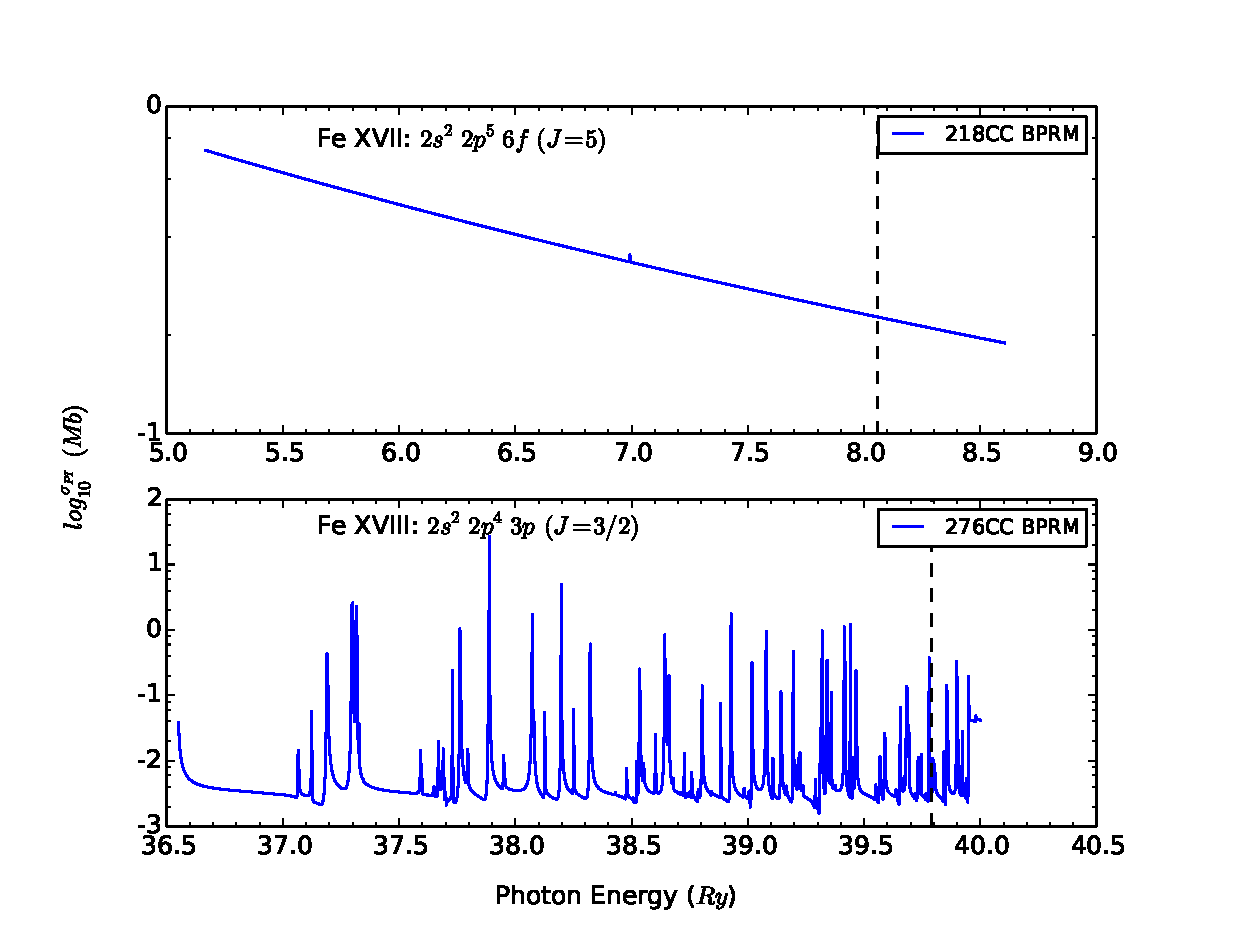
\includegraphics[width=.9\textwidth]{figures_chap_4/negative_region}	
	\caption{The averaged photoionization cross section below the lowest threshold. Dashed vertical line indicates the lowest threshold position.}
	\label{figure_negative_region}
\end{figure}

\subsection{The Ground State of Fe XVII}
The 99LS-RM calculation is done by \citet{99cc_2016}, and the ground state is singlet, i.e. no fine structure, thus this level is not splitted and should match with the one in 218 CC-BPRM calculation. In figure \ref{figure_bound_99_218}, we may easily find that below the lowest threshold, there are many resonances for 218CC-BPRM calculation, but no resonances in 99LS-RM. Though the energy mesh in 218CC-BPRM calculation is about as 10 times dense as the one used in 99LS-RM, there is still a chance that 99LS-RM does not give resonances in this region. Above the lowest threshold, the two results agree very well, but at the tail of 99LS-RM calculation, there are oscillations, which might be due to the insufficient number of continuum basis functions used (see Section \ref{sec_nrang2_oscillation}). 

%======= FIGURE: negative region
\begin{figure}
	\centering
	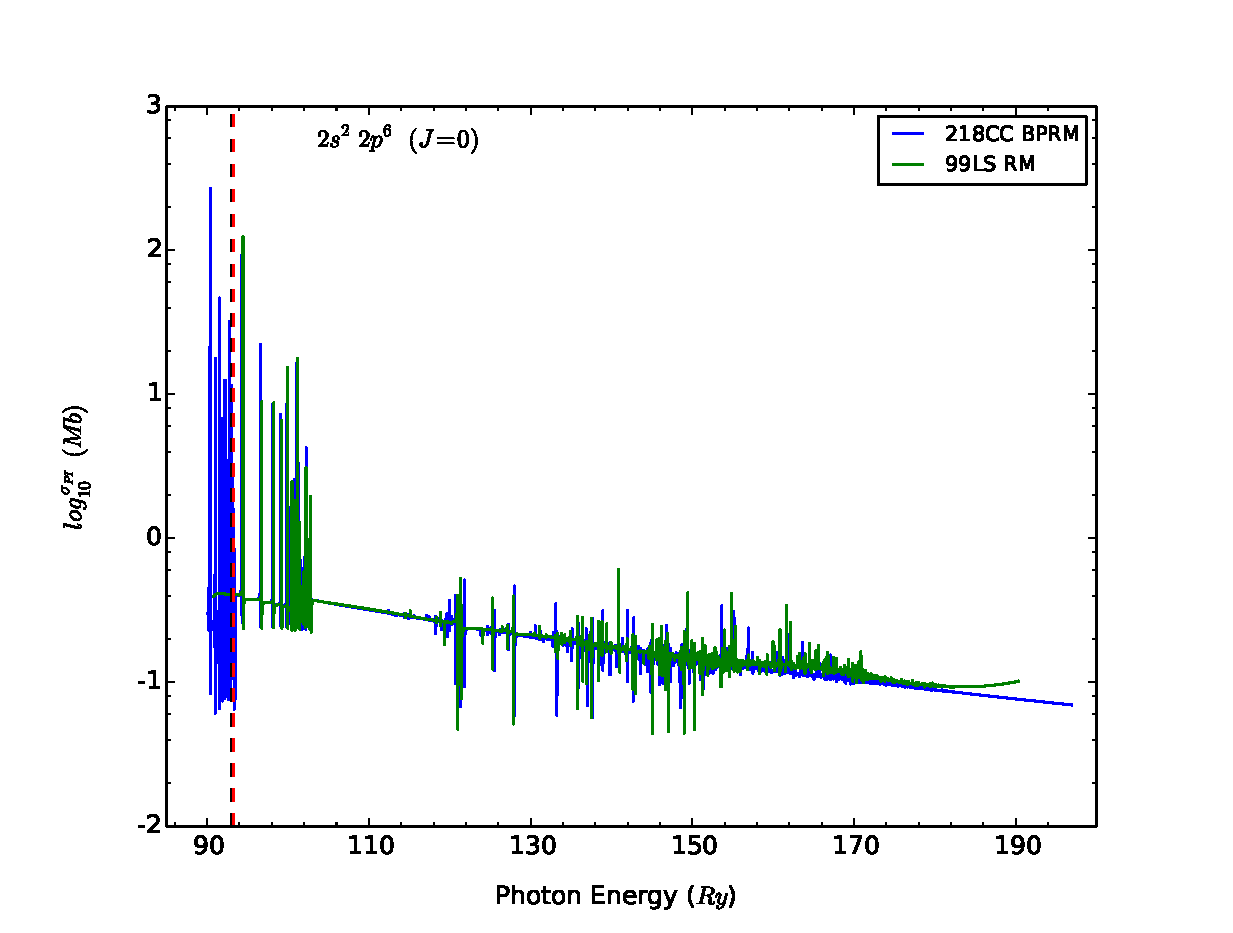
\includegraphics[width=.9\textwidth]{figures_chap_4/fe17_ground_99_218}	
	\caption{The ground state of \ion{Fe}{xvii} in 99LZ-RM and 218 CC-BPRM. The dashed line is the lowest threshold. Black: 218CC-BPRM; red: 99LS-RM. }
	\label{figure_bound_99_218}
\end{figure}


\subsection{MAXC/NRANG2 and Oscillation} \label{sec_nrang2_oscillation}
In the current calculation, the number of continuum basis functions used is 20, which turns out to be insufficient, as it causes oscillations in the photoionization cross section, especially for the high-symmetry bound states (see figure \ref{figure_oscillation}). In figure \ref{figure_oscillation}, we can see that this oscillation happens not only in the high energy region, but also in the lower part, maybe in the middle too. We remove the tail of such oscillations for all states in our opacity calculation (see Chapter \ref{chap_topup}). To overcome this, we may need to increase the number of continuum basis functions, however, this will cause the Hamiltonian matrix size to increase exponentially, thus making the computation extremely hard.
%======= FIGURE: oscillation
\begin{figure}
	\centering
	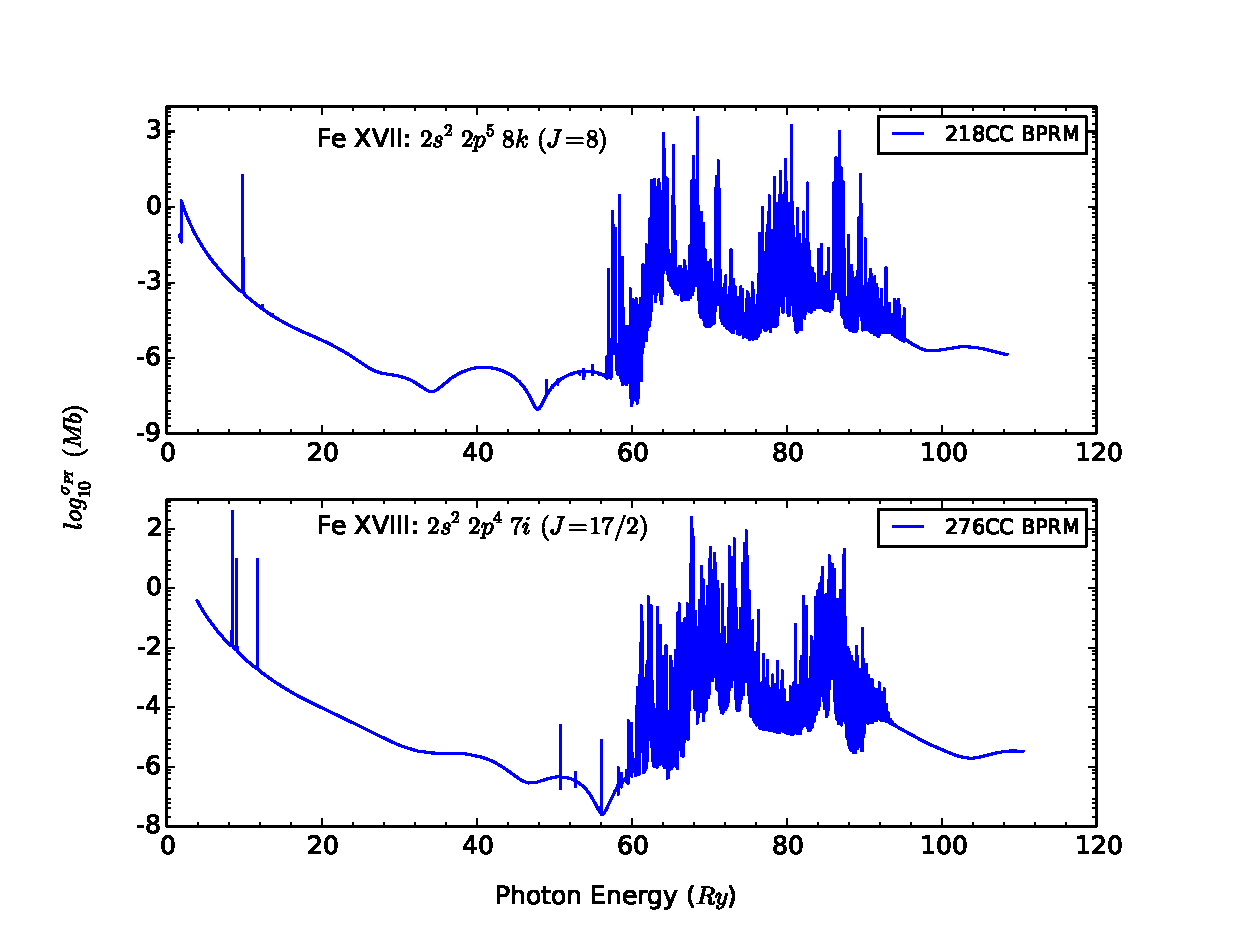
\includegraphics[width=.9\textwidth]{figures_chap_4/oscillation}	
	\caption{The severe oscillations in the photoionization cross section due to small number of continuum basis functions.}
	\label{figure_oscillation}
\end{figure}

\subsection{Resonances}
One of the most salient features of the close coupling approximation is the autoionization resonances due to the coupling between open and closed channels. In the left part of figure \ref{figure_resonance_theory} it  shows a few possible energy levels formed by the core $N$-electron system, and in the right part of the figure, it shows schematically some of the bound levels fomed by coupling each state of the core with an outer electron and these levels just lie below each corresponding core state level. Since we define the ground state of the core having energy of 0, all the bound levels below 0 are purely bound levels, while the levels above are quasi-bound levels. So in BPRM calculation, bound-bound transitions are denoted by A only below 0 energy. While bound-free transitions are between levels below 0 energy line and the ones above 0. There are two kinds of bound-free atomic processes. One is direct photoionization described by open channels, which means the electron is directly photoionized, and the final state is not on the quasi-bound lines. The other is photo-excitation followed by autoionization described by closed channels, and the intermediate state on one of these quasi-bound lines, e.g. a, which can be formed by core state i or other higher core states. Since level a is quasi-bound state, core i can undergo a transition to a lower level, e.g. f1 or f2, without radiation. According to the conservation of energy, the (N+1)th electron now has a positive energy relative to f1 or f2, thus ionized and free. In the following we outline the procedures used to incorporate the resonances.

%======= FIGURE: resonance theory
\begin{figure}
	\centering
	\includegraphics[width=.9\textwidth]{figures_chap_4/resonances_theory}	
	\caption{A diagram showing the bound-bound transitions (A), direct photionization process (B) and photo-excitation-autoionization process (C) treated in BPRM calculation.}
	\label{figure_resonance_theory}
\end{figure}

Define the projection operators $P$ and $Q$ where $P$ projects onto the subspace spanned by the open channels and $Q$ onto the orthogonal subspace, then the Schr\"odinger equation \ref{eq_schodinger} can be rewritten as
\begin{align}
	P(H-E)(P+Q) \Psi_a = 0 \\
	Q(H-E)(P+Q) \Psi_a = 0
\end{align}
, which may be combined into
\begin{equation} \label{eq_resonances}
	P\Bigg(H-PHQ\frac{1}{Q(H-E)Q}QHP-E\Bigg)P\Psi_a = 0
\end{equation}
Define the eigenfunctions of $QHQ$ as 
\begin{equation}
	QHQ\zeta_j = \varepsilon_j\zeta_j
\end{equation}
The second term in equation \ref{eq_resonances} is the optical potential and corresponds to the scattered electron propogating in the orthogonal space $Q$ and it can be expressed as
\begin{equation}
	V_{opt} = \sum_{j=1,m}|PHQ\zeta_j\rangle\frac{1}{\varepsilon_j-E}\langle\zeta_jQHP|
\end{equation}
, so the resonances are due to the poles in $V_{opt}$. 
In the close coupling approximation, the resonances can be due to the closed channels in the expansion \ref{eq_full_expand}. In this case, we can write
\begin{align}
	P\psi_k(x_1\cdot\cdot\cdot x_{N+1}) &= \mathcal{A}\sum_{i}^{NO}\overline{\Phi}_i(x_1\cdot\cdot\cdot x_{N}; \hat{\textbf{r}}_{N+1}\sigma_{N+1}) \frac{1}{r_{N+1}} F_{ik}(r_{N+1}) \\
	Q\psi_k(x_1\cdot\cdot\cdot x_{N+1}) &= \mathcal{A}\sum_{NO+1}^{n}\overline{\Phi}_i(x_1\cdot\cdot\cdot x_{N}; \hat{\textbf{r}}_{N+1}\sigma_{N+1}) \frac{1}{r_{N+1}} F_{ik}(r_{N+1})
\end{align}
, or it can be due to the short-range correlation terms, so in this case, we can write
\begin{align}
	P\psi_k(x_1\cdot\cdot\cdot x_{N+1}) &= \mathcal{A}\sum_{i}^{NO}\overline{\Phi}_i(x_1\cdot\cdot\cdot x_{N}; \hat{\textbf{r}}_{N+1}\sigma_{N+1}) \frac{1}{r_{N+1}} F_{ik}(r_{N+1}) \\
	Q\psi_k(x_1\cdot\cdot\cdot x_{N+1}) &= \sum_{j=1}^m d_{jk} \chi_j(x_1\cdots x_{N+1}) 
\end{align}
In some cases this may cause pseudo-resonances due to inappropriate choose of correlation configurations \citep{pseudo_reso_1, pseudo_reso_2}.

%======= FIGURE: resonances
\begin{figure}
	\centering
	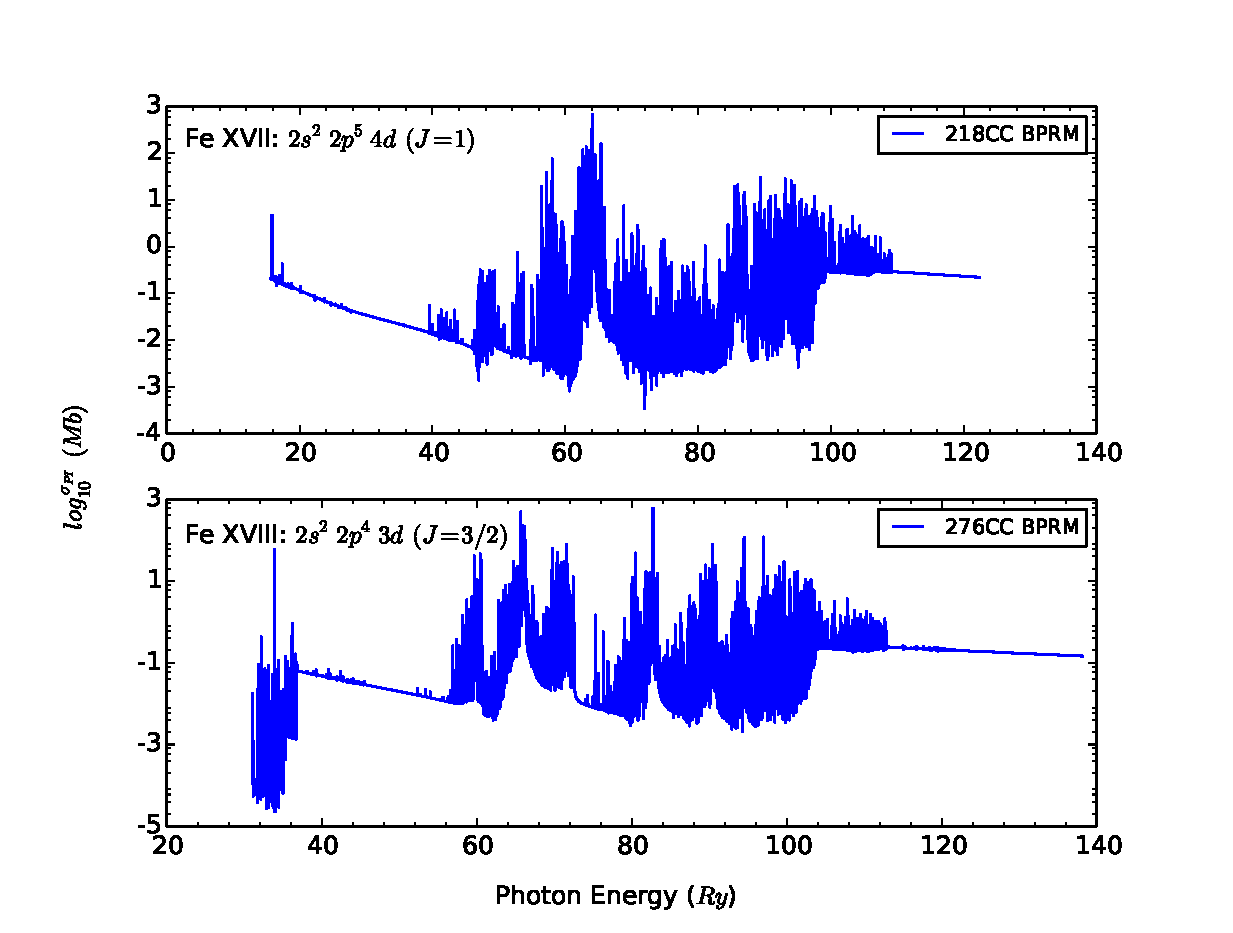
\includegraphics[width=.9\textwidth]{figures_chap_4/resonances}	
	\caption{Rydbeg resonances and PEC.}
	\label{figure_resonances}
\end{figure}

Among the narrow Rydberg resonances, there are considerably broader resonances with greater magnitude, which are called PEC resonances. They are mainly due to the photoexcitation of the core (PEC), where the excitation only occurs in the target leaving the outer electron as a spectator, and these transitions are strong dipole-allowed, i.e. wavefunctions have a considerable radial overlap which was very well studied in \citet{opcd_4} and \citet{pec_2}. In figure \ref{figure_resonances}, we can observe such resonances with very wide width and large magnitude, which modify the photoionization cross section considerably.

\section{Conclusion}
In this chapter, we outlined the formulae used to calculate the radiative data, i.e. oscillator strength and photoionization cross section. we provided the key parameters used in the current BPRM calculations, and gave a brief study on the photoionization cross section just the lowest threshold, the comparison of the ground state of \ion{Fe}{xvii} for 99LS-RM and 218CC-BPRM calculations, the effects of NRANG2 on the data and also the standard Rydberg resonances and PEC resonances. We believe the current calculation gives more accurate atomic data, though improvements can be made on the larger number of continuum basis functions to eliminate the oscillations in the lower energy region.



